\documentclass[../main.tex]{subfiles}
\graphicspath{{img/}}
\begin{comment}
    Introduction. State (1) the purpose of the investigation, (2) the problem being investigated, (3) the background (context and importance) of the problem (citing previous work by others), (4) your thesis and general approach, and (5) the criteria for your study's success.

    Theory. Develop the theoretical basis for your design or experimental work, including any governing equations. Detailed calculations go to an appendix.
\end{comment}
\begin{document}
In Fisica gli esperimenti ad alte energie sono quelli che rendono possibile investigare i fenomeni che avvengono nelle parti remote dell'Universo, conoscere i comportamenti delle particelle e ricreare le condizioni in cui l'Universo si trovava nei primi istanti della sua vita. Per esempio, si realizzano esperimenti di collisione di fasci di particelle in cui le particelle accelerate vengono fatte scontrare su un bersaglio, per poi rilevare e analizzare i prodotti della collisione. Oppure, si tenta di intercettare i prodotti degli eventi ad alte energie che già avvengono nel nostro universo, come le esplosioni di stelle o le collisioni di buchi neri. In particolare i neutrini, particelle debolmente interagenti, attraversano l'universo conservando l'informazione dell'evento che li ha generati. Proprio per questo però la loro rilevazione è estremamente ardua. L'esperimento europeo KM3Net si propone di farlo sfruttando la radiazione Cherenkov emessa dalle particelle cariche relativistiche generate dalla fortuita interazione tra i neutrini cosmici e l'acqua o i fondali marini. L'apparato dell'esperimento consiste in centinaia di unità ottiche distribuite in un volume di un \SI{}{\km ^3} e ancorate al fondale del Mar Adriatico al largo delle coste di Sicilia, Francia e Grecia (\autoref{fig:towers}). Ciascuna unità ottica comprende 31 fotomoltiplicatori (PMT).

\begin{figure}[h!b]
    \centering
    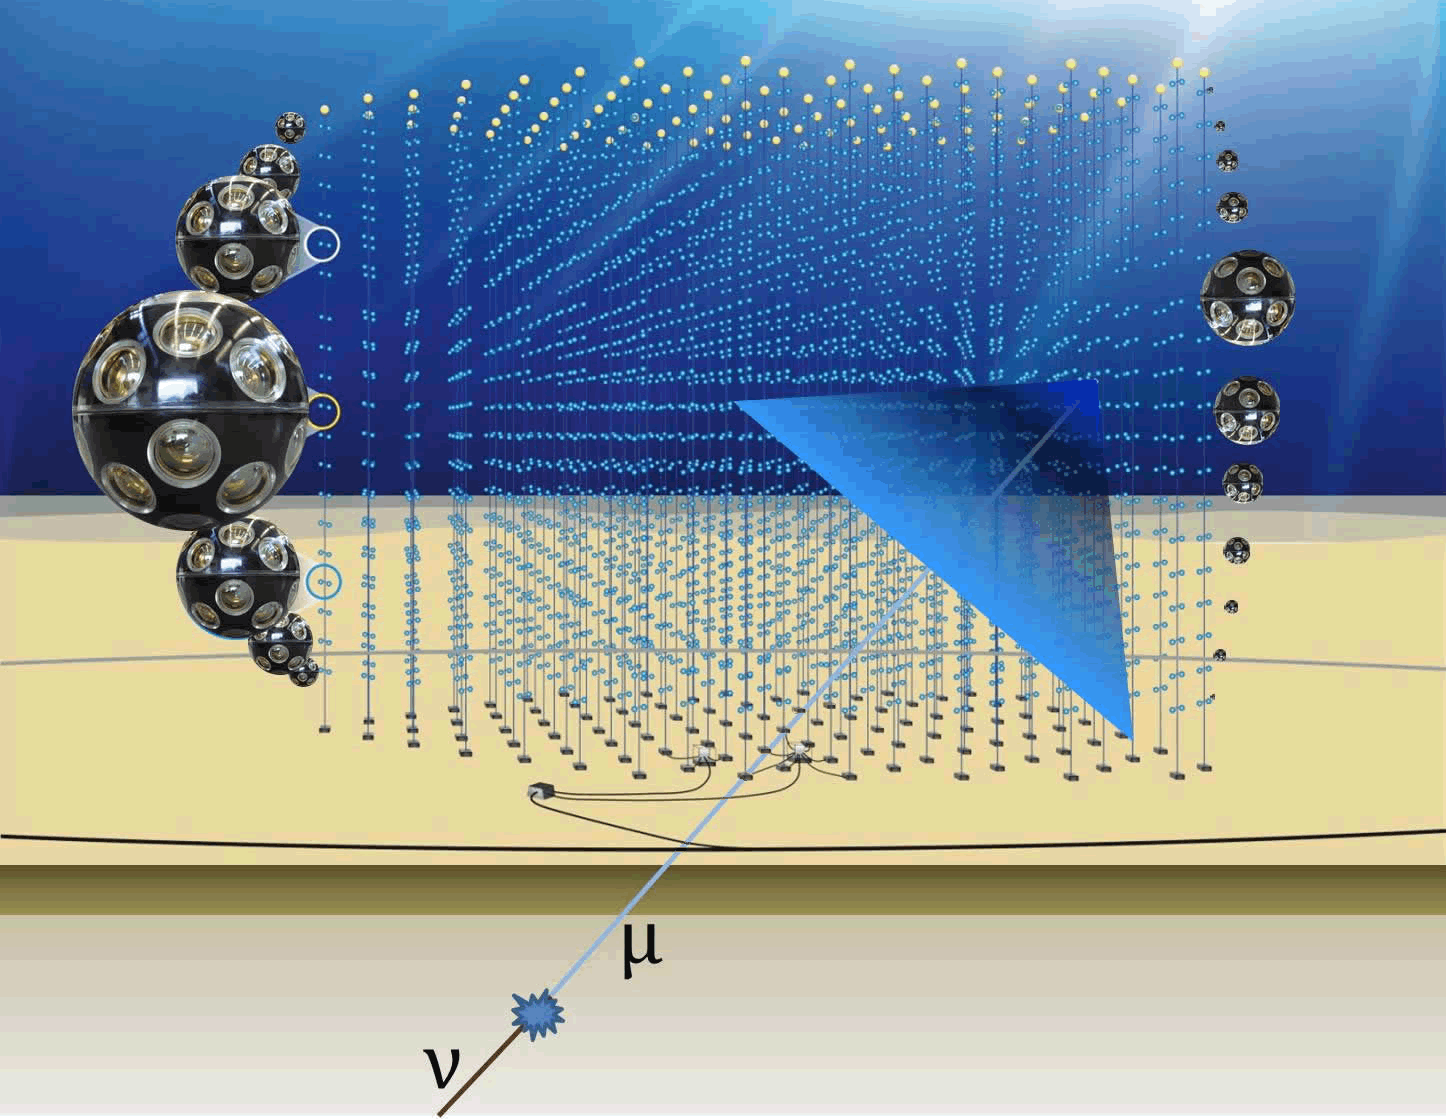
\includegraphics[width=0.6\textwidth]{KM3NetTowers.png}
    \caption{\small Centinaia di torri di 18 unità ottiche ciascuna ancorate al fondale e sostenute da un galleggiante vanno a formare l'installazione di KM3Net. Quando un neutrino interagisce con la materia terrestre in prossimità del volume del rilevatore, viene generato un muone che produce un cono di luce per effetto \emph{Cherenkov}, il quale viene rilevato dalle unità ottiche. Quindi la traiettoria del neutrino e la posizione celeste dell'evento che lo ha generato vengono ricostruiti.
    \cite{km3}}
    \label{fig:towers}
\end{figure}

L'intero apparato genera quindi un flusso di dati di circa \SI{30}{GBps}, anche a causa del rumore di fondo come il decadimento di ${}^{40}K$, il quale va necessariamente filtrato attraverso un \emph{trigger}, ovvero impostando una soglia di energia o sfruttando le coincidenze temporali date dalla fisica del fenomeno, affinché sia possibile memorizzare e analizzare i dati. Se solitamente questa operazione avviene via hardware direttamente nel luogo di installazione dei sensori, in questo caso la locazione sottomarina impone un approccio \emph{all-data-to-shore}, dove il flusso di dati è trasmesso a terra e quindi processato via software. A questo scopo è stato sviluppato TriDAS (Trigger and Data Acquisition System), un sistema \emph{triggerless} (che non prevede, appunto, un trigger hardware) di acquisizione e filtraggio di dati.

Con l'aumento delle capacità dei sistemi di calcolo diventa sempre più comune implementare sistemi \emph{triggerless} via software. Per esempio, presso i \emph{Jefferson Lab}, centro di ricerca statunitense di fisica nucleare (Newport News, Virginia) TriDAS è stato utilizzato nel 2020 per processare i dati di un esperimento di collisione di fascio di elettroni. TriDAS prevede anche la possibilità di inserire altri livelli di trigger definiti dall'utente, caratteristica che lo rende molto versatile. Questo lavoro ha come scopo l'implementazione di un livello di trigger che, nell'ambito di un esperimento di collisione di fascio, escluda dall'acquisizione quei segnali provenienti da fonti diverse dal fascio, in particolare da raggi cosmici.


Nel primo capitolo si mostra una breve descrizione degli esperimenti di collisione di fascio e del funzionamento dei rilevatori comunemente utilizzati.
Il secondo capitolo mostra la struttura e il funzionamento del software TriDAS.
Quindi nel terzo capitolo si descrive come il trigger è stato implementato, i metodi usati per testarlo, l'apparato sperimentale su cui è stato testato e i risultati ottenuti.
Infine si commentano i risultati.

\end{document}
